
%--------------------------------------------------------------------
% Document Style
%--------------------------------------------------------------------
% Save LaTeX kernel version of \@xfloat





\documentclass[12pt]{report}
\usepackage{smu_thesis}






\usepackage{epsf}
\usepackage{amsmath,bm}
\usepackage{graphicx}
\usepackage{verbatim}
\usepackage{algorithm}
\usepackage{algorithmic}
\usepackage{fancyhdr}

\usepackage{multirow}
\usepackage{url}

\usepackage[justification=centering]{caption} 

\usepackage{subfigure}
%\usepackage{subcaption}


\renewcommand{\algorithmicrequire}{\textbf{Input:}}
\renewcommand{\algorithmicensure}{\textbf{Output:}}
\renewcommand{\baselinestretch}{0.94}


\linespread{1.6}
%\thesisdraft

\begin{document}

%===================================================================
%   Change information used to create front pages of thesis
%===================================================================
%%
%%  last name, first name, initial
%%
 \Name{Cui}{Pengfei}{} %don't put anything in the last brackets

%%
%% title -- you have up to three lines to specify your title
%% each line should be no more than 48 characters long
%%
 \Title{Exploiting Spectrum Agility in Wireless Links and Networks}
       { }
       { }
%%
%% previous degress
%%
 \DegreeA{B.S., Beijing Institute of Technology, 2007}
 \DegreeB{M.S., University of Chinese Academy of Sciences, 2010}
%%
%% degree you are seeking
%%
 \DegreeSought{Doctor of Philosophy}
%%
%% major
%%
 \Major{Electrical Engineering}
 \University{Southern Methodist University}
 \School{Bobby B. Lyle School of Engineering}
%%
%% date the degree will be confered
%%
 \DegreeDate{TBA}
 \ThesisDate{TBA}
%%
%% is this a thesis, dissertation, or something else?
%%
 \ThesisType{Dissertation}
%%
%% your committee -- the rank of your advisor must be adjusted in
%% smu_thesis.sty if it is not Dr.
%%
 \Advisor{Joseph Camp}
 \CommitteeMemberA{Dr. Dinesh Rajan}
 \CommitteeMemberB{Dr. Eli Olinick}
 \CommitteeMemberC{Dr. Carlos Davila}
 \CommitteeMemberD{Dr. Panos Papamichalis}


%===================================================================
%   Create the front pages of the thesis
%===================================================================

 \ApprovalTitlePages

%%
%% include your acknowledgements
%% If no dedication, move Acknowledgement to where dedication is and add to
%% table of contents
%% \addcontentsline{toc}{chapter}{\protect \noindent {ACKNOWLEDGMENTS}}
 \begin{Acknowledgment}
 \input{acknow}
 \end{Acknowledgment}

%%
%% include your abstract
%%
 \begin{Abstract}
 \begin{abstract} 

The emergence of the reapportioned white space bands for data usage will fuel the already
increasing frequency band diversity of today's wireless hardware. As a result, many
existing multi-channel and/or multi-band adaptation schemes will become more important.
Many of these works have considered the capacity and channel activity of these channels,
but have not distinguished between the propagation characteristics that occur when considering
a difference in frequency of multiple GHz and the resulting effect in various environments.
In this paper, we leverage the contextual information and propagation diversity to enable
adaptation across a number of frequency bands from 700 MHz to 5.8 GHz.  To do so, we
perform a number of experiments in a vehicular environment using a campus bus.  With a
model based on a Support Vector Machine (SVM) and an in-situ training set, we can predict
the throughput on a free channel.  We can then consider the activity level per band to 
compute the net throughput we should expect on a given band to guide our adaptation protocol.  
In the field, we exploit the propagation differences experience per band to show that training on a repeatable 
route can yield vast performance improvements from prior schemes.  We show that minimal  
amounts of training can provide such improvements and that a simple scheme that can allow
multiband adaptation gains when there is insufficient levels of training.


%Probably at this time we could not employ the bus doing the experiments.

%Unused spectrum whitespaces in the currently underutilized analog TV bands are able to exploit for future wireless networks. There are potential room for performance improvement of wireless communication in throughput, power consumption and link fairness extending wireless to these bands. Previous methods are focused on channel adaptation across multiple channels in one band without considering the propogation and other characters among different bands. In this work, we employ the propogation difference for performance prediction of multiband adaptation. To identify the crowded level,we involve an activity level of networks based on the statistics information during a time slot to make the prediction more accuracy. The amount of context information required for multiband adaptation and the influerence of window size for activity level are evaluated in this paper. We conduct indoor and in-field experiments to validate our method. The experimental results demonstrate that our method is able to achieve as ... 


\end{abstract}



 \end{Abstract}

 \PreliminaryPages

% Uncomment to insert a list of symbols from symbols.tex (or elsewhere)
 %\begin{listofsymbols}
 %\input{symbols}
 %\end{listofsymbols}

%%
%% include your dedication
%%
 \Dedicate{}

%===================================================================
%   Begin the body of the thesis
%===================================================================
\begin{thesis}
%===================================================================
%   Chapters are included here
%===================================================================

\input{chap_intro.tex}
\input{chap_background.tex}
\chapter{In-field Measurements} 
\label{ch:measurements}

In this chapter, we describe the background of our research, 
including the basic technology related to this work, the 
hardware and software tools that we used to implement and evaluate 
our proposed algorithms in this work.


\section{White Space Bands}



\chapter{Vehicular Link Spectrum Adaptation} 
\label{ch:vnc}

%
\section{Introduction}
\label{sec:introduction}


%Background
%Worldwide governments and societies are active to achieve road safety and travel comfort of drivers and passengers.
Drivers and passengers around the world could utilize a wide array of vehicular applications ranging from real-time traffic monitoring and
safety applications to various {\it infotainment} applications.
%spanning news, weather, audio, and video streams.  
However, the continuous use of such applications is limited due to the challenge of transmitting over 
highly-dynamic vehicular wireless channels. 
In such networks, the increasing availability of different 
frequency bands with correspondingly diverse propagation characteristics could allow flexibility and 
robustness of vehicular links. Even with spectral flexibility, links are extremely tenuous, 
demanding instantaneous decisions to remain connected, motivating an algorithm that
can find the appropriate frequency band quickly and according to the current environmental context.

Cognitive radio mechanisms which interleave channel accesses also motivate the frequency
band selection problem of finding the optimal spectrum on which to 
transmit~\cite{ghasemi2008spectrum}.
%Furthermore, in existing systems, there are a number of different technologies from which to choose and the demand of
% integrating the advantages of multiple protocol is presented as Heterogeneous Wireless Networks has opening topics related to band selection~\cite{hossain2010vehicular}.
Prior work has considered a number of challenges in
leveraging white space frequencies including spectrum sensing, frequency-agile operation,
geolocation, solving stringent spectral mask requirements, and providing reliable service
in unlicensed and dynamically changing spectrum~\cite{shellhammer2009technical}. In particular, there has recently been an acceleration
in spectrum sensing work~\cite{rayanchu2011fluid, kim1996pulse,cabric2004implementation}. Based on 
these works, protocols have been built for multi-channel and/or multiband wireless operation~\cite{MOAR,
raychaudhuri2003spectrum,sabharwal2007opportunistic}.  Other works have presented methods for searching for the most efficient 
transmission channel~\cite{mo2005comparison}, discovering channel information~\cite{rayanchu2011fluid, sabharwal2007opportunistic}, and estimating 
channel quality~\cite{MOAR}.
Finally, the emergence of a number of diverse sensors on a vehicle motivates work
on heterogeneous wireless networks, which have different frequency bands {\it and}
technologies~\cite{hossain2010vehicular}. Thus, the various communication 
standards have diverse throughput capacity, allowing the choice of technology 
to possibly usurp frequency band decisions. For example, an 802.11n link at 5.8 
GHz with high levels of loss
might still be a better choice than a Bluetooth link at 2.4 GHz with little loss
due to the discrepancy of hundreds of Mbps in throughput capacity.
%To consider the choice of frequency band, band selection problem for htereogeneous wireless networks should be researched under the same protocol, which make it similar to our problem~\cite{hossain2010vehicular}.
%Add heterogeneous and cognitive radio
%Research of heterogeneous wireless networks has been done for these purpose in Roadside-to-Vehicle and Vehicle-to-Vehicle.\cite{hossain2010vehicular}.
%the understanding of primary/secondary users adaptation\cite{cordeiro2007c}, combining multiple devices for vehicle~\cite{hossain2010vehicular}.

However, for the purposes of this work, we assume the underlying technology is the same to evaluate the choice of frequency band.
While these works have considered spectral activity and developing protocols and algorithms to 
find spectral holes, less of a focus has been on coupling such information with historical performance in a given 
propagation environment.
In this paper, 
we develop multiband adaptation protocols which couple the prior knowledge of in-situ performance of various bands with the instantaneous knowledge of 
spectral activity, SNR, and current location of each band to arrive at a decision on the optimal band to transmit. To do so, we use an
off-the-shelf platform that allows direct comparison and simultaneous experimentation across four different wireless
frequency bands from 450 MHz to 5.8 GHz with the same physical
and media access layers. 
%changes that frequency differences of hundreds of MHz to GHz could have on the band %decision. Moreover, it is well known that propagation greatly depends on the environment %in operation~\cite{rappaport}.  Thus, knowledge of the environment in operation could %allow the relationship between received power differences across multiple frequency bands %to have much greater accuracy.  

%Contributions  fixme
The main contributions of our work are as follows:
\begin{itemize}
\item We first develop a framework for multiband adaptation using both historical information and instantaneous measurements. This framework is broad enough to study adaptation across licensed and unlicensed bands, including white space frequency bands.  

\item We propose two different machine-learning-based multiband adaptation algorithms. The 
first machine learning algorithm, referred to as the \emph{Location-based 
Look-up Algorithm}, 
is based on the idea of $k$-nearest-neighbor classification. The second machine-learning-based 
algorithm uses \emph{decision trees} for classification. 
For comparison, we also create two baseline adaptation algorithms which attempt to make the optimal band selection based on only: (i.)~historical 
performance data, and (ii.)~instantaneous SNR measurements across 
various bands. 

%We consider four different algorithms for comparison.  First, we consider a scheme
%in which the throughput is achieved on an emulated channel for
%the current received signal level. We then adjust the predicted best band choice according to the current activity
%level (real-time information). 
%Second, we consider an approach based on machine learning which
%considers prior throughput for a given received signal and activity level
%combination.  
%Third, we build a scheme which include the prior relationship of throughput, received signal level and context information in an look up table for repeatable travel in an area.
%Fourth, we split the area to different regions and apply machine learning in each region to get the property band selection.

%earning in addition to the received signal and activity level.
%Third, we consider a second machine learning approach which considers user
%location in addition to the received signal and activity level.

\item We perform extensive outdoor V-2-V experiments to evaluate the proposed algorithms.
Our results indicate that the proposed machine learning based algorithms improve
throughput by up to $49.3\%$ over these baseline methods.

\end{itemize}



%The remainder of this paper is organized as follows. In Section II, we present the multiband adaptation problem and proposed algorithms. Section III discusses experimental evaluation of the multiband algorithms. We conclude in Section IV.




In this section, we first formulate the multiband 
adaptation problem in vehicular wireless links and introduce the set of information we use to make band decisions, which we refer to as context information. We then propose two machine-learning-based 
multiband adaptation algorithms for vehicular channels. For comparison, we also propose two baseline adaptation methods based on existing solutions which consider historical and instantaneous information independently.




\section{Link Adaptation Problem Formulation}
%The focus of this paper is on a context-based multiband adaptation algorithm as:
%The problem we are going to resolve is to find a band has the best throughput in multiple available options as:

Consider a system with~$n$ frequency bands, represented by an index set~$\{1,2, \ldots, n\}$. 
The objective is to select the optimal band,~$b_{best}$, to transmit at each time instant that maximizes a desired objective function such as throughput. The throughput~$r_i$ on band~$i$ depends on several factors such as received signal power~$P_R^i$, noise power~$P_N^i$, the channel activity level~$A^i$, the velocity of the transmitter,~$v_{tx}$,
 the velocity of the receiver,~$v_{rx}$, 
 and location information which depends on each algorithm and will be specified in the algorithm section. The aforementioned set of all information used to make multiband decisions composes the users context. 
 %Add Context
% Context is the information that can represent the characters of a wireless user.For mobile wireless users, velocity, RSSI, interference and location could be counted as context information.
This relationship is represented in general as~$r_i = f(P_R^i, P_N^i, A^i, v_{tx}, v_{rx}, $context information per algorithm$)$. The objective can be stated as:
\begin{equation}
b_{best}= \arg \max_i r_i 
\end{equation}
The framework differentiates interference from other nodes using the same technology (via the Activity level $A^i$) and other technologies (via the noise level~$P_N^i$). For instance, an 802.11 node can decode the packets of other 802.11 nodes but can only sense
instantaneous noise levels from ZigBee/Bluetooth nodes. 
Decoding the packets can provide increased knowledge such as 
data rate and packet size to determine the duration of the channel use.
%To help make decisions for multiband adaptation in a similar context,
We can exploit the long-term behavior by using historical performance
data for the collected context information
({\it e.g.}, $v_{tx}$, $v_{rx}$, $A^i$, $P_N^i$, $P_R^i$)~\cite{meikle2012global}. 
%can be used by people tending to have repeatable patterns
%~\cite{meikle2012global} and we could improve the performance with each trip 
%to the region if we could passively observe context along this repeatable 
%pattern. The variables used in each algorithm will be explained for each algorithm 
%later. 


%To represent the utilization level of the channel, we define \emph{activity level}, $A$,
%as the percentage of time when the channel is occupied by 
%all competing sources $x_j (j = 1, 2, 3, ...)$ other than the intended transmitter $y$. 
%For 802.11-based transmissions, the activity level on band $i$ is defined as:
%\begin{equation}
%\label{eqn:80211activity}
%A^i = \frac{\sum_j{\sum_k{\frac{L_k^{x_j}}{R_k^{x_j}}}}}{\sum_k{\frac{L_k^y}{R_k^y}}+\sum_j{\sum_k{\frac{L_k^{x_j}}{R_k^{x_j}}}}+S\sigma}
%\end{equation}
%where $L_k^{x_j}$ and $R_k^{x_j}$ represent the packet length in bits and data
%rate at which that packet is transmitted, for external sources $x_j$;
%$S$ and $\sigma$ are the number of idle slots and slot duration, respectively. 
%When considering the activity level of non-802.11 users 
%({\it e.g.}, the bands currently licensed to TV),
%we use the received signal level from non-802.11 interfering sources $P_N^i$ 
%on band $i$ directly as an input to our algorithms. 

\section{Multiband Adaptation Algorithms}
\label{subsec:algorithms}

In order to evaluate the proposed multiband adaptation algorithms, 
we construct two baseline methods: (i.) We search for the
most commonly selected band as the best band in the historical data
and choose it as the final band decision. (ii.) For each band, we build 
a lookup table for throughput $T_{ideal}$ in an idealized channel given the $RSSI$ and obtain 
the best band according to following:
\begin{align}
&\max_i\ T_{ideal}^i\times(1-A^i),
\label{eq:baseline2}
\end{align}
The throughput $T_{ideal}$ is measured with an Azimuth ACE-MX channel emulator~\cite{AzimuthACE}. 
The details of the system setup and data collection are discussed in Section~\ref{sec:vncexperimentdesign}. 

Machine learning has been used as an important tool in wireless communications~\cite{haykin2005cognitive}. When a user enters an area, the machine
learning algorithm can learn from the historical data and
select the potential optimal band given the input, {\it e.g.}, $P_R^i$, $v$
and $P_N^i$. We propose two multiband adaptation algorithms based on
two machine learning methods: k-nearest neighbor (KNN) and decision trees.

%2 machine learning methods: 
%1. modified KNN, 

{\bf Location-based Look-up Algorithm.} KNN is a machine learning method
based on searching for the closest training data points in the feature space and various
modified versions have been applied successfully for classification~\cite{zhang2006svm}.
In the {\it Location-based Look-up Algorithm}, we search for the closest neighbors of 
a testing point by using each parameter one by one in the input set. 
The {\it Location-based Look-up Algorithm} additionally involves geographic information for band selection other than received signal power~$P_R^i$, noise power~$P_N^i$, the activity/occupancy level~$A^i$, the velocity of the transmitter,~$v_{tx}$.
The 
performance of the selected training data points is averaged to generate an estimate of the performance at each band. Then
the band with the highest throughput performance is selected as $b_{best}$.
%comparing with machine learning algorithms. 

For the {\it Location-based Look-up Algorithm}, 
context information involves the location $g$ (GPS latitude and longitude), $v$, $P_R^i$, $P_N^i$ 
and $A^i$. To make a band prediction, we have four look-up blocks to reduce
the training data points which are similar to the testing data point. First,
we search for the historical data which is closest to the testing data based on GPS location.
If the number of found historical data points is less than a predefined threshold, 
 $\theta_{AArea}$, we increase the distance range (the actual threshold is discussed in 
Section~\ref{sec:vncexperimentdesign}). Then, based on the filtered historical data,
we collect $\theta_{AArea}$ data points which are closest to $P_R^i$, where $\theta_{AArea}$ is the threshold of the number of collected data points. 
A similar process is repeated based on $P_N^i$ and $v$, respectively.
After deciding the final data set, we average the throughput of data points at each band.
This algorithm's key steps are shown in Algorithm~\ref{algorithms: Location}.


\begin{algorithm}
\caption{Location-based Look-up Algorithm}
\label{algorithms: Location}
\begin{algorithmic}[1]
\REQUIRE  ~~\\
	 $g$: Location information of multiband node\\
	 $\theta_{Area}$: Threshold of a location\\
	 $\theta_{RSSI}$: Threshold of RSSI\\
	 $\theta_{Velocity}$: Threshold of velocity\\
	 $\theta_{set} = \{\theta_{A Area},\theta_{A RSSI},\theta_{A Non 802.11 SI},\theta_{A Velocity}\}$: Threshold of data amount for \{a location, RSSI, non-802.11 interference, velocity\}\\
%	 $\theta_{A Area}$: Threshold of data amount for a location\\
%	 $\theta_{A RSSI}$: Threshold of data amount for RSSI\\
%	 $\theta_{A Non 802.11 SI}$: Threshold of data amount for non-802.11 interference\\
%	 $\theta_{A Velocity}$: Threshold of data amount for velocity\\
	 $D^i \in \{D^1,D^2,\dots,D^n\}$: Historical look-up data
\FOR    {$i<=n$}
\STATE Initialize \emph{$Data_{Location}, Data_{RSSI}, Data_{Velocity}$} to zero matrix;


\FOR {$j<=m$}
\STATE $Amount = Amount_{\{Data_{Location,i},Data_{RSSI,i},Data_{P_N,i},Data_{Velocity,i}\}}^j$;
\STATE $\theta = \theta_{set}^j$;
\WHILE {$Amount<\theta$}
\STATE $Data_{Location,i} \leftarrow f_{Lookup}(D^i,g,\theta_{Area})$: Find data in $D^i$ whose distance less than $\theta_{Area}$;
\STATE $\theta_{Area}=\theta_{Area} \times 1.1$;
\ENDWHILE

%\WHILE {$Amount(Data_{RSSI,i})<\theta_{A RSSI}$}
%\STATE $Data_{RSSI,i} \leftarrow f_{Look-up}(D_{Location,i},P_R^i,\theta_{RSSI})$: Find data in $D_{Location}$ the RSSI similar to $P_R^i$ in range $\theta_{RSSI}$;
%\STATE $\theta_{RSSI}=\theta_{RSSI} \times 1.1$;
%\ENDWHILE
%
%\WHILE {$Amount(Data_{P_N,i})<\theta_{A Non 802.11 SI}$}
%\STATE $Data_{RSSI,i} \leftarrow f_{Look-up}(D_{Location,i},P_N^i,\theta_{RSSI})$: Find data in $D_{Location}$ the RSSI similar to $P_N^i$ in range $\theta_{RSSI}$;
%\STATE $\theta_{A Non 802.11 SI}=\theta_{A Non 802.11 SI} \times 1.1$;
%\ENDWHILE

%\WHILE {$Amount(Data_{Velocity,i})<\theta_{A Velocity}$}
%\STATE $Data_{Velocity,i} \leftarrow f_{Lookup}(D_{RSSI,i},v,\theta_{Velocity})$: Find data in $D_{RSSI}$ the RSSI similar to $v$ in range $\theta_{RSSI}$;
%\STATE $\theta_{Velocity}=\theta_{Velocity} \times 1.1$;
%\ENDWHILE \\

\STATE $T_{a,i}=avr(Data_{Velocity,i})$;
\STATE  $T_{e,i}=T_a^i\times(1-A^i)$;
% ENDFOR for amount and theta
\ENDFOR \\  
\ENDFOR \\  
\STATE $b_{best} = \max_i\{T_e^1,\dots,T_e^i,\dots,T_e^n\}$;\\
\ENSURE ~~\\    
$b_{best}$: Optimal transmission band
\end{algorithmic}
\end{algorithm}

%2. region-based C4.5 (different region sizes)
{\bf Region-based Decision Tree Algorithm.} Decision trees are a  
widely-used machine learning 
algorithm due to their low complexity and stable performance~\cite{banfield2007}.
A decision tree can model the relationship in the training data between the context 
information and the optimal band as a set of tree-like deduction structures. Before 
implementing the training process, we prepare a training set including a group of 
training data points of $\{v_{tx}, v_{rx}, P_R^1, ..., P_R^n,  A^1, ..., A^n, P_N^1, 
..., P_N^n, b_{best}\}$ based on the collected measurements. We obtain $b_{best}$ by comparing
the throughput performance of all available bands and selecting the band with the highest 
throughput. We choose the C4.5 algorithm to generate our decision tree~\cite{hall2009weka}, a widely-used algorithm based on the 
information entropy gain. 

At each intermediate
node in the decision tree, the learning algorithm calculates the information entropy 
gain of splitting the remaining training data points based on each parameter in the input 
set, {\it e.g.}, $P_R^i$, $v$ or $P_N^i$. Then, it compares and selects the parameter with 
the highest entropy gain to decide the test condition at each intermediate node until 
all training data points are classified.  The leaf nodes indicate the optimal band for 
prediction in our application. Then, the trained decision structure is integrated into 
the transmitter protocol stack. With the collected context information, the decision 
structure can suggest the band with the best throughput performance. 

The relationship between the context information and the best band could differ at
different locations because of diverse propagation environment characteristics. 
To reduce the heterogeneity of training data from different locations, we split 
the vehicular route into several regions and implement the training process based 
on the historical data collected in each region. Then, the trained decision structure 
is integrated in our system for multiband adaptation in each region. The granularity 
of regional division is one parameter that affects the training set as well as the 
performance of the resulting decision tree. We 
evaluate the granularity of these divisions in Section~\ref{sec:vncexperimentdesign}.

\section{Experiments for Multiband Algorithms}
\label{sec:vncexperimentdesign}

%As discussed in Section \ref{subsec:algorithms}, 
%one algorithm is applicable for entering a strange area, 3 algorithms are more appropriate for area has been visited.
To study these algorithms, we have developed indoor 
and in-field experiments on 
%an off-the-shelf wireless platform.
%Testbed and emulator Platform
%To ensure the results are broadly applicable, we employ 
a Linux-based 802.11 testbed~\cite{Openwrt}. The platform includes a 
Gateworks 2358 motherboard with Ubiquiti XR radios (XR9 at 900 MHz, 
XR2 at 2.4 GHz, XR5 at 5.2 GHz) and a DoodleLabs DL475 radio at 
450 MHz~\cite{Gateworks,Ubnt}.  We use 
an Azimuth ACE-MX channel emulator for
controllable propagation and fading characteristics with a broad range of 
industry-standard channel models from 450 MHz to 5.9 GHz~\cite{AzimuthACE}. 

%context information experiments
\subsection{In-lab Experiments for Radio Characterization}
\label{subsec:ichannel}
To establish an SNR-to-throughput relationship for the \emph{SNR-based 
Throughput Look-up Algorithm}, we use an experimental setup where two 
wireless nodes communicate across repeatable emulated channels generated 
by the channel emulator (Figure~\ref{fig:in-door experiment}). For a given band and card, we measure
the throughput of a fully-backlogged UDP flow using the {\it iperf} 
traffic generator. We use constant attenuation over an idealized
channel condition and repeat the experiment to
produce various RSSI values.
Despite the same physical and media access control layers of the radios, there are
slight differences in the throughput achieved per radio at the same attenuation
level.  Thus, we normalize these throughput values to have the same maximum
throughput across radio types.
%for a fair comparison of the frequency bands.

\begin{figure} [h]
%\vspace{-0.1in}
\centering
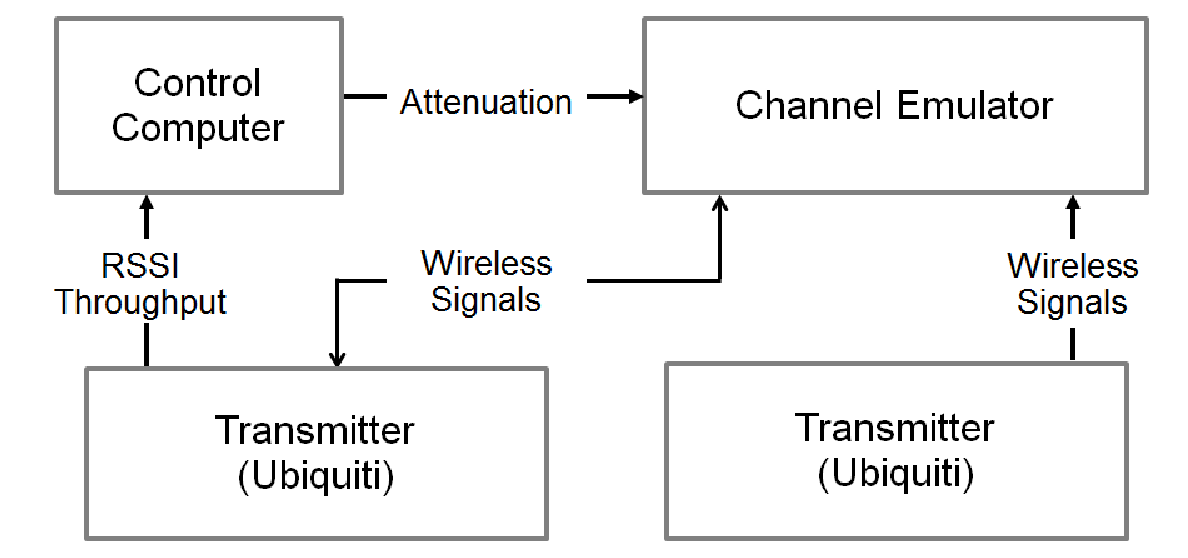
\includegraphics[width=85mm]{figures/emulator2}
%\vspace{-0.1in}
\caption{Experimental setup for channel emulator.}
\label{fig:in-door experiment}
\vspace{-0.1in}
\end{figure}

%\subsection{Signal Level Context-aware information}
\subsection{Experimental Design for In-field Data Collection}
\label{subsec:insitu}
We now describe the in-field experimental design to obtain a data set for
evaluating our multiband algorithms. Two Gateworks boards, each containing
the aforementioned four radios, are installed on two cars.  One node is always
the receiver and at a fixed location. The other node is always the 
transmitter and travels 
around the block of a public park as shown in Figure~\ref{fig:infield}.
One loop of the route will be used as a unit of training in the next section.

\begin{figure} [h]
%\vspace{-0.1in}
\centering
\includegraphics[width=85mm]{figures/infield}
\vspace{-0.1in}
\caption{In-field Experimental Setup.}
\label{fig:infield}
\vspace{-0.1in}
\end{figure}

During each loop, the transmitter sends a fully-backlogged UDP flow
using {\it iperf} on each of the four radios simultaneously.  To
focus on band selection and ensure the greatest range, we disable autorate and use a fixed data rate
of 6 Mbps. The receiver continually performs a {\it tcpdump} of all
received 802.11 packets~\cite{jacobson1989tcpdump}. Additionally, a
QH 400 Quad Ridge Horn Antenna (shown in Figure~\ref{fig:infield}) is 
connected to a Rhode \& Schwarz FSH8 mobile spectrum analyzer at the 
receiver to monitor spectral activity. Then, based on the 
time stamps, we remove 802.11 packets from the spectral trace 
so that only non-802.11 interference will contribute to $P_N^i$.

\begin{figure} 
%\vspace{-0.1in}
\centering
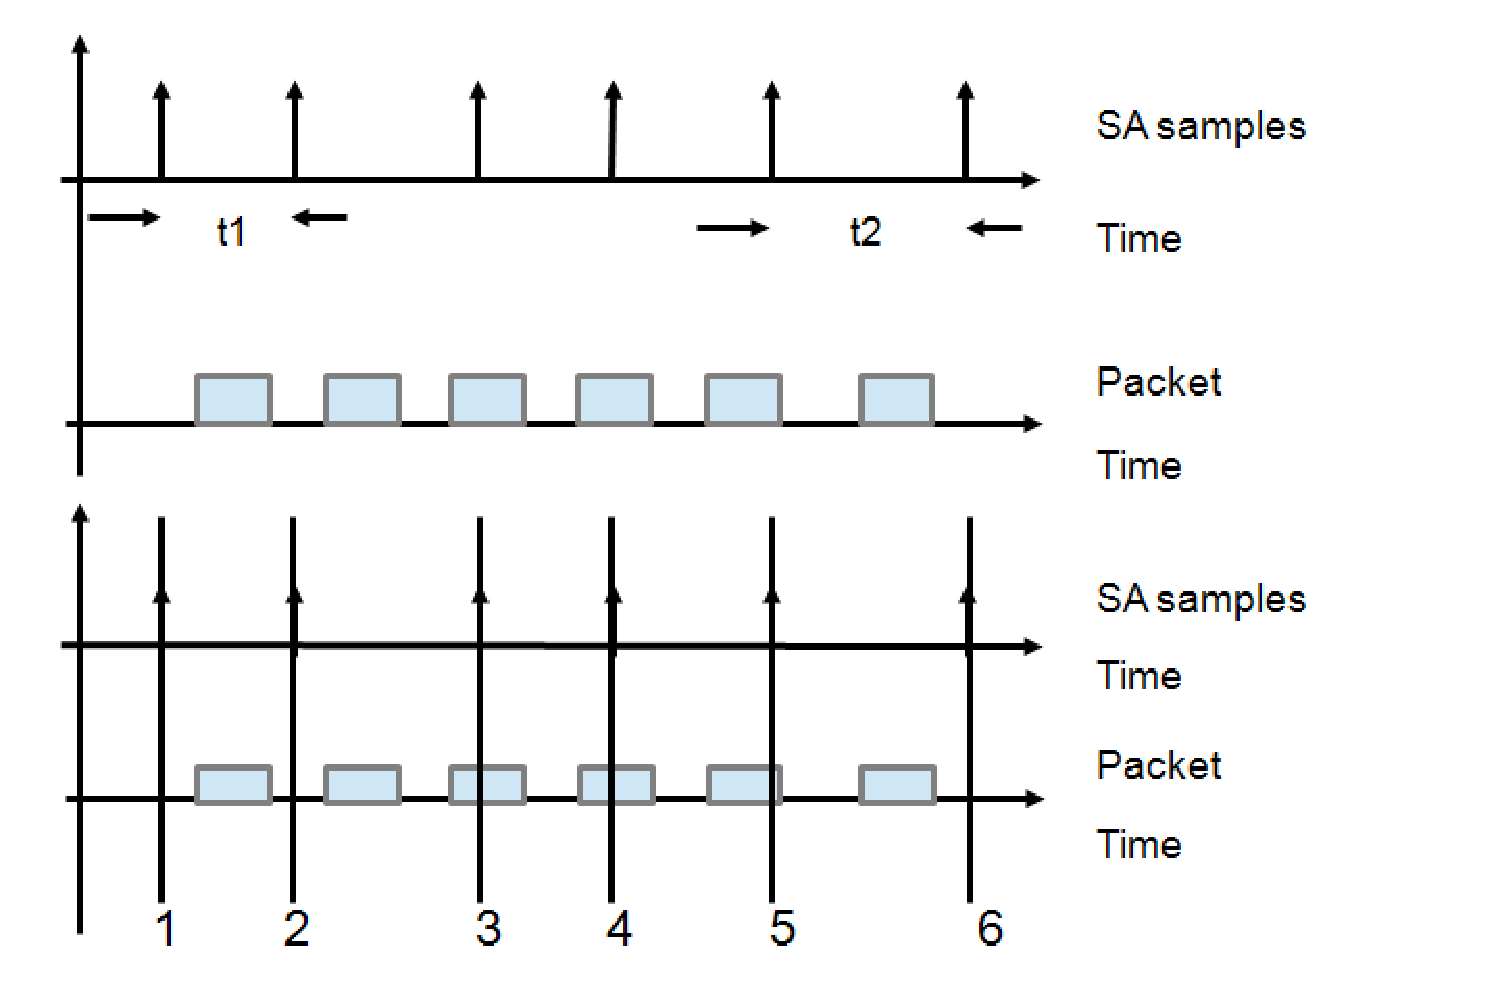
\includegraphics[width=85mm]{figures/sa_process}
\vspace{-0.1in}
\caption{Spectrum Analyzer Data Processing.}
\label{fig:sa_process}
\vspace{0.1in}
\end{figure}

Figure~\ref{fig:sa_process} shows how we obtain the
non-802.11 interference, $P_N^i$. We expunge the spectrum analyzer
(SA) samples which overlap in time with the dumped 802.11 packets,
such as packets 3, 4, and 5. Then, the reported interference value
will not contain the received power from 802.11 packets, which have
already been considered via the activity level, $A$.

The in-field data is processed offline where data from all instruments
involved is synchronized based on the GPS time stamps. 
As discussed in Section~\ref{subsec:ichannel}, the throughput of each radio
is normalized based upon emulator experiments to account for any
manufacturing differences.


\section{Data Process}
\label{sec:experiment}

Fixme


%Detail may not useful
Parsing script
In our experiments, we are constantly collecting large amounts of data, including the received signal level, current location, velocity, and time of day. Working with the memory-limited Gateworks boards, it became necessary to implement a solution to collect large amounts of data without exhausting the available memory space on the boards. Thus, we compiled a script to parse an undetermined number of data files containing the raw data collected from the ongoing experiments. Utilizing the Perl programming language, which the Gateworks boards are capable of running, the script scans every file in a directory we specify and parses them, looking specifically for signal level, lat/long location, velocity, and time data recorded from the experiments. Upon finding this information, the script reformats the data by placing it into a .csv file. Additionally, using the location data, the script calculates the  distance between the transmitting and receiving boards and adds this information to the .csv file. Upon parsing the data, the raw experimental data files can simply be delete from memory, freeing up space for the data of subsequent experiments.

Activity monitor script
For in-situ experiments, the need became apparent to track the number of new incoming packets and compare it with the number of previously received packets. Additionally, this needed to be done for each of the four wireless radios on the board. In doing this, we identify the most efficient frequency band to transmit data. To implement this system, a script was needed to run efficiently in the background while experiments were taking place. To achieve this, we wrote a bash shell script to run directly on the board without relying on any higher level programming language that could potentially cause greater performance overhead. As a result, the script only consumes one to two percent of CPU resource. The script begins by examining the received bytes across each radio for a length of 30 seconds and placing the bytes received each second on a new line in a file. Upon the completion of the 30 second buffering time period, the next second of received bytes on each radio is read and compared with the last 30 seconds of received data. This ratio of the most recent received data to old received data is then calculated and written to four files, one for each radio, for its subsequent use in selecting which radio to transmit/receive from.


%\section{Related Work}
\label{sec:related}

Cognitive Radio could be a powerful tool for the utility of the Spectrum Opportunity~\cite{haykin2005cognitive}.
Analog TV bands will be released for wireless communication brings opportunity to combine current wireless bands and new available bands for performance improvement employing Cognitive Radio methods~\cite{MOAR}. 


%Related research
A bunch of work has been done on radio-scene analysis and channel identification for utility of channel adaptation dating back to Simon Haykin~\cite{haykin2005cognitive}.
Some work of Multi-bands/Multi-channels in
cognitive radios focus on optimize performance, such as avoiding frequency diversity~\cite{rahul2009frequency}. 
In~\cite{OAR} an opportunistic algorithm is introduced to balance the cost of spectrum sensing, channel switching and the gain of these activities.


%Our work
Our work is motivated by prospective releasing band used for TV now and exploit the comparison across all the available bands in the future. 
It is an extension of multi-channel adaptation. 
Most of the published research focus on the stopping rules of spectrum sensing~\cite{sabharwal2007opportunistic, OAR}. In contrast, we use the data and framework to classify the performance across different bands based on the parameters we get from the context information.
%{\bf .} 


\section{Summary}
\label{sec:vncsummary}


In this chapter, we investigated multiband adaptation to leverage the propagation and context for vehicular applications. 
We did so by proposing two machine-learning-based schemes and compared their
performance against two baseline schemes.
In our experimental analysis, we evaluated the performance of these algorithms 
in the field on an off-the-shelf platform.
Experimental results demonstrate that the proposed algorithms can 
achieve up to 49.3\% greater throughput than the baseline algorithms
with an accuracy up to 65\%. In future work, we will study the impact that
multiple diverse environments have on the training as well as evaluate
the optimal use of multiple, diverse radios in unison.
%Since mobile networks have limited
%energy and training in multiple environment has not been investigated, in future work we plan to examine the influence of diverse environment and energy efficiency of
%the simultaneous use of multiple, diverse radios.



\chapter{Spectrum Adaptation for Single Hop Access Networks} 
\label{ch:winmee}

% Introduce the content of this section
In this chapter, we illustrate the challenges of band selection
in wireless network deployments and formulate the problem of band 
selection in wireless network deployments jointly using WiFi and white space bands. 
Further, we present a measurement-driven framework for estimating the 
access point number to serve the traffic demand of a given population.


\input{multiband_winmee/problemformulation}
\section{Data Process}
\label{sec:experiment}

Fixme


%Detail may not useful
Parsing script
In our experiments, we are constantly collecting large amounts of data, including the received signal level, current location, velocity, and time of day. Working with the memory-limited Gateworks boards, it became necessary to implement a solution to collect large amounts of data without exhausting the available memory space on the boards. Thus, we compiled a script to parse an undetermined number of data files containing the raw data collected from the ongoing experiments. Utilizing the Perl programming language, which the Gateworks boards are capable of running, the script scans every file in a directory we specify and parses them, looking specifically for signal level, lat/long location, velocity, and time data recorded from the experiments. Upon finding this information, the script reformats the data by placing it into a .csv file. Additionally, using the location data, the script calculates the  distance between the transmitting and receiving boards and adds this information to the .csv file. Upon parsing the data, the raw experimental data files can simply be delete from memory, freeing up space for the data of subsequent experiments.

Activity monitor script
For in-situ experiments, the need became apparent to track the number of new incoming packets and compare it with the number of previously received packets. Additionally, this needed to be done for each of the four wireless radios on the board. In doing this, we identify the most efficient frequency band to transmit data. To implement this system, a script was needed to run efficiently in the background while experiments were taking place. To achieve this, we wrote a bash shell script to run directly on the board without relying on any higher level programming language that could potentially cause greater performance overhead. As a result, the script only consumes one to two percent of CPU resource. The script begins by examining the received bytes across each radio for a length of 30 seconds and placing the bytes received each second on a new line in a file. Upon the completion of the 30 second buffering time period, the next second of received bytes on each radio is read and compared with the last 30 seconds of received data. This ratio of the most recent received data to old received data is then calculated and written to four files, one for each radio, for its subsequent use in selecting which radio to transmit/receive from.


\input{multiband_moa/problemformulation}
\section{Data Process}
\label{sec:experiment}

Fixme


%Detail may not useful
Parsing script
In our experiments, we are constantly collecting large amounts of data, including the received signal level, current location, velocity, and time of day. Working with the memory-limited Gateworks boards, it became necessary to implement a solution to collect large amounts of data without exhausting the available memory space on the boards. Thus, we compiled a script to parse an undetermined number of data files containing the raw data collected from the ongoing experiments. Utilizing the Perl programming language, which the Gateworks boards are capable of running, the script scans every file in a directory we specify and parses them, looking specifically for signal level, lat/long location, velocity, and time data recorded from the experiments. Upon finding this information, the script reformats the data by placing it into a .csv file. Additionally, using the location data, the script calculates the  distance between the transmitting and receiving boards and adds this information to the .csv file. Upon parsing the data, the raw experimental data files can simply be delete from memory, freeing up space for the data of subsequent experiments.

Activity monitor script
For in-situ experiments, the need became apparent to track the number of new incoming packets and compare it with the number of previously received packets. Additionally, this needed to be done for each of the four wireless radios on the board. In doing this, we identify the most efficient frequency band to transmit data. To implement this system, a script was needed to run efficiently in the background while experiments were taking place. To achieve this, we wrote a bash shell script to run directly on the board without relying on any higher level programming language that could potentially cause greater performance overhead. As a result, the script only consumes one to two percent of CPU resource. The script begins by examining the received bytes across each radio for a length of 30 seconds and placing the bytes received each second on a new line in a file. Upon the completion of the 30 second buffering time period, the next second of received bytes on each radio is read and compared with the last 30 seconds of received data. This ratio of the most recent received data to old received data is then calculated and written to four files, one for each radio, for its subsequent use in selecting which radio to transmit/receive from.




\input{multiband_whitecell/problemformulation}
\input{multiband_whitecell/problemstatement}
\section{Data Process}
\label{sec:experiment}

Fixme


%Detail may not useful
Parsing script
In our experiments, we are constantly collecting large amounts of data, including the received signal level, current location, velocity, and time of day. Working with the memory-limited Gateworks boards, it became necessary to implement a solution to collect large amounts of data without exhausting the available memory space on the boards. Thus, we compiled a script to parse an undetermined number of data files containing the raw data collected from the ongoing experiments. Utilizing the Perl programming language, which the Gateworks boards are capable of running, the script scans every file in a directory we specify and parses them, looking specifically for signal level, lat/long location, velocity, and time data recorded from the experiments. Upon finding this information, the script reformats the data by placing it into a .csv file. Additionally, using the location data, the script calculates the  distance between the transmitting and receiving boards and adds this information to the .csv file. Upon parsing the data, the raw experimental data files can simply be delete from memory, freeing up space for the data of subsequent experiments.

Activity monitor script
For in-situ experiments, the need became apparent to track the number of new incoming packets and compare it with the number of previously received packets. Additionally, this needed to be done for each of the four wireless radios on the board. In doing this, we identify the most efficient frequency band to transmit data. To implement this system, a script was needed to run efficiently in the background while experiments were taking place. To achieve this, we wrote a bash shell script to run directly on the board without relying on any higher level programming language that could potentially cause greater performance overhead. As a result, the script only consumes one to two percent of CPU resource. The script begins by examining the received bytes across each radio for a length of 30 seconds and placing the bytes received each second on a new line in a file. Upon the completion of the 30 second buffering time period, the next second of received bytes on each radio is read and compared with the last 30 seconds of received data. This ratio of the most recent received data to old received data is then calculated and written to four files, one for each radio, for its subsequent use in selecting which radio to transmit/receive from.




\section{Summary}
\label{sec:winmeeconclusion}

In this chapter, we jointly considered the use of WiFi and white space bands for 
deploying wireless access networks across a broad range of population densities.
To consider network deployment costs, we proposed a Multiband Access Point Estimation 
framework to find the number of access points required in a given region.
We then performed spectrum utilization measurements in the DFW metropolitan 
and surrounding areas to drive our framework and find the influence of white spaces on
network costs in these representative areas. Through 
extensive analysis across varying population density and channel combinations across bands, 
we show that white space bands can reduce the number of access points by 1650\%
and 660\% in rural and sparse urban areas, respectively. However, the same cost savings
are not achieved in dense urban and downtown type area. Finally, we investigate different 
band combinations in two population densities to show that greater access to white space 
channels have greater total savings of mesh nodes when the total number of channels used 
in the network is fixed (i.e., given a total number of allowable WiFi and white space channels). 
As the population and spectrum utilization increase, the cost savings of white space bands
diminish to the point that WiFi-only channel combinations can be optimal.
Through extensive analysis across varying population density and channel combinations 
across bands, we show that white space bands application in hetergeneous access point 
can reduce the number of access points by 260\% in sufficient white space configuration
and 80\% gain in limited white channel scenarios.
% Whitecell
To consider the power consumption of a system, we 
formulate the heterogeneous wireless network as a queuing system. 
We then analyze the heterogeneous queuing system based on previous queuing 
theory work. To address the resource allocation of white space channels, 
we proposed a Greedy Server-side Replace algorithm to find the resource allocation 
with minimum power consumption. We then perform spectrum utilization 
measurements in the typical areas of downtown, urban, campus, neighborhoods 
to drive the algorithm. We also leverage the user mobility pattern from WiEye 
measurements. Through extensive analysis across the spectrum utilization 
and user mobility, we show that white space bands can reduce the average of 
power consumption by 64.70\% on average over 24 hours. We also integrated previous 
measurements work in north Texas and find the power consumption is reduced by white space
bands by 512.55\% in sparse area.
In the future, we will consider to propose the heterogeneous wireless network 
deployment with large scale user mobility patterns.
% Future work




\chapter{Spectrum Adaptation for Multihop Access Networks} 
\label{ch:wm}


\input{multiband_wm/problemformulation}
\input{multiband_wm/linearopt}
\input{multiband_wm/wmalgorithms}
\section{Data Process}
\label{sec:experiment}

Fixme


%Detail may not useful
Parsing script
In our experiments, we are constantly collecting large amounts of data, including the received signal level, current location, velocity, and time of day. Working with the memory-limited Gateworks boards, it became necessary to implement a solution to collect large amounts of data without exhausting the available memory space on the boards. Thus, we compiled a script to parse an undetermined number of data files containing the raw data collected from the ongoing experiments. Utilizing the Perl programming language, which the Gateworks boards are capable of running, the script scans every file in a directory we specify and parses them, looking specifically for signal level, lat/long location, velocity, and time data recorded from the experiments. Upon finding this information, the script reformats the data by placing it into a .csv file. Additionally, using the location data, the script calculates the  distance between the transmitting and receiving boards and adds this information to the .csv file. Upon parsing the data, the raw experimental data files can simply be delete from memory, freeing up space for the data of subsequent experiments.

Activity monitor script
For in-situ experiments, the need became apparent to track the number of new incoming packets and compare it with the number of previously received packets. Additionally, this needed to be done for each of the four wireless radios on the board. In doing this, we identify the most efficient frequency band to transmit data. To implement this system, a script was needed to run efficiently in the background while experiments were taking place. To achieve this, we wrote a bash shell script to run directly on the board without relying on any higher level programming language that could potentially cause greater performance overhead. As a result, the script only consumes one to two percent of CPU resource. The script begins by examining the received bytes across each radio for a length of 30 seconds and placing the bytes received each second on a new line in a file. Upon the completion of the 30 second buffering time period, the next second of received bytes on each radio is read and compared with the last 30 seconds of received data. This ratio of the most recent received data to old received data is then calculated and written to four files, one for each radio, for its subsequent use in selecting which radio to transmit/receive from.


%\section{Related Work}
\label{sec:related}

Cognitive Radio could be a powerful tool for the utility of the Spectrum Opportunity~\cite{haykin2005cognitive}.
Analog TV bands will be released for wireless communication brings opportunity to combine current wireless bands and new available bands for performance improvement employing Cognitive Radio methods~\cite{MOAR}. 


%Related research
A bunch of work has been done on radio-scene analysis and channel identification for utility of channel adaptation dating back to Simon Haykin~\cite{haykin2005cognitive}.
Some work of Multi-bands/Multi-channels in
cognitive radios focus on optimize performance, such as avoiding frequency diversity~\cite{rahul2009frequency}. 
In~\cite{OAR} an opportunistic algorithm is introduced to balance the cost of spectrum sensing, channel switching and the gain of these activities.


%Our work
Our work is motivated by prospective releasing band used for TV now and exploit the comparison across all the available bands in the future. 
It is an extension of multi-channel adaptation. 
Most of the published research focus on the stopping rules of spectrum sensing~\cite{sabharwal2007opportunistic, OAR}. In contrast, we use the data and framework to classify the performance across different bands based on the parameters we get from the context information.
%{\bf .} 


\section{Summary}
\label{sec:vncsummary}


In this chapter, we investigated multiband adaptation to leverage the propagation and context for vehicular applications. 
We did so by proposing two machine-learning-based schemes and compared their
performance against two baseline schemes.
In our experimental analysis, we evaluated the performance of these algorithms 
in the field on an off-the-shelf platform.
Experimental results demonstrate that the proposed algorithms can 
achieve up to 49.3\% greater throughput than the baseline algorithms
with an accuracy up to 65\%. In future work, we will study the impact that
multiple diverse environments have on the training as well as evaluate
the optimal use of multiple, diverse radios in unison.
%Since mobile networks have limited
%energy and training in multiple environment has not been investigated, in future work we plan to examine the influence of diverse environment and energy efficiency of
%the simultaneous use of multiple, diverse radios.


%%\chapter{Multiband Hetegeneous Access Point Optimization} 
%\label{ch:moa}


\input{multiband_moa/problemformulation}
\section{Data Process}
\label{sec:experiment}

Fixme


%Detail may not useful
Parsing script
In our experiments, we are constantly collecting large amounts of data, including the received signal level, current location, velocity, and time of day. Working with the memory-limited Gateworks boards, it became necessary to implement a solution to collect large amounts of data without exhausting the available memory space on the boards. Thus, we compiled a script to parse an undetermined number of data files containing the raw data collected from the ongoing experiments. Utilizing the Perl programming language, which the Gateworks boards are capable of running, the script scans every file in a directory we specify and parses them, looking specifically for signal level, lat/long location, velocity, and time data recorded from the experiments. Upon finding this information, the script reformats the data by placing it into a .csv file. Additionally, using the location data, the script calculates the  distance between the transmitting and receiving boards and adds this information to the .csv file. Upon parsing the data, the raw experimental data files can simply be delete from memory, freeing up space for the data of subsequent experiments.

Activity monitor script
For in-situ experiments, the need became apparent to track the number of new incoming packets and compare it with the number of previously received packets. Additionally, this needed to be done for each of the four wireless radios on the board. In doing this, we identify the most efficient frequency band to transmit data. To implement this system, a script was needed to run efficiently in the background while experiments were taking place. To achieve this, we wrote a bash shell script to run directly on the board without relying on any higher level programming language that could potentially cause greater performance overhead. As a result, the script only consumes one to two percent of CPU resource. The script begins by examining the received bytes across each radio for a length of 30 seconds and placing the bytes received each second on a new line in a file. Upon the completion of the 30 second buffering time period, the next second of received bytes on each radio is read and compared with the last 30 seconds of received data. This ratio of the most recent received data to old received data is then calculated and written to four files, one for each radio, for its subsequent use in selecting which radio to transmit/receive from.


%\section{Related Work}
\label{sec:related}

Cognitive Radio could be a powerful tool for the utility of the Spectrum Opportunity~\cite{haykin2005cognitive}.
Analog TV bands will be released for wireless communication brings opportunity to combine current wireless bands and new available bands for performance improvement employing Cognitive Radio methods~\cite{MOAR}. 


%Related research
A bunch of work has been done on radio-scene analysis and channel identification for utility of channel adaptation dating back to Simon Haykin~\cite{haykin2005cognitive}.
Some work of Multi-bands/Multi-channels in
cognitive radios focus on optimize performance, such as avoiding frequency diversity~\cite{rahul2009frequency}. 
In~\cite{OAR} an opportunistic algorithm is introduced to balance the cost of spectrum sensing, channel switching and the gain of these activities.


%Our work
Our work is motivated by prospective releasing band used for TV now and exploit the comparison across all the available bands in the future. 
It is an extension of multi-channel adaptation. 
Most of the published research focus on the stopping rules of spectrum sensing~\cite{sabharwal2007opportunistic, OAR}. In contrast, we use the data and framework to classify the performance across different bands based on the parameters we get from the context information.
%{\bf .} 


%\section{Summary}
\label{sec:vncsummary}


In this chapter, we investigated multiband adaptation to leverage the propagation and context for vehicular applications. 
We did so by proposing two machine-learning-based schemes and compared their
performance against two baseline schemes.
In our experimental analysis, we evaluated the performance of these algorithms 
in the field on an off-the-shelf platform.
Experimental results demonstrate that the proposed algorithms can 
achieve up to 49.3\% greater throughput than the baseline algorithms
with an accuracy up to 65\%. In future work, we will study the impact that
multiple diverse environments have on the training as well as evaluate
the optimal use of multiple, diverse radios in unison.
%Since mobile networks have limited
%energy and training in multiple environment has not been investigated, in future work we plan to examine the influence of diverse environment and energy efficiency of
%the simultaneous use of multiple, diverse radios.


\input{chap_related.tex}
%
% Introduce the content of this section
The objective of the mesh network deployment is to minimize the number of 
deployed mesh nodes with the network constraints. In this section we first 
describe the the motivation of frequency agility in mesh network deployment. 
Then we propose a graph-theoretic model for the network deployment problem
with the QoS constraints of an operational wireless mesh network.

% Problem
In our previous work, we address the link communication spectrum adaptation, 
single hop access network deployment, and the multihop access network channel
assignment. Next, we are going to answer the question how to locate the mesh
network access nodes and gateways in multiband spectrum adaptation scenario.
The input of the problem is a target service area given with the parameters 
such as population distribution, spectrum usability, and FCC licensed channels, 
etc. The output is to locate the network infrastructure from the candidates.
Thus, the target area with pre-defined parameters could be modeled as a 
connectivity graph with vertices represented as the centralized traffic demand 
of a certain area and potential access points locations. The edges denote the 
links between the locations. Oppose to previous works,
~\cite{robinson2010deploying,franklin2007node,tang2005interference,irwin2013resource}
we formulate the input connectivity graph as a graph $G = (V,E,F)$, where centralized
traffic demand, access points location candidates and links from a type of access 
point defined by its frequency form a unified connectivity graph. 
We are searching for the output of the problem which is expected to be an graph 
$G' = (V',E',F')$ marks the mesh, gateway nodes and chosen frequency for them. 

The vertices in the modeled input graph represent a set $C$ of  separated target 
area with traffic demands. The set $C$ consists of physical coordinates representing 
target areas where client coverage is desired, analogous to the area to be covered 
in a geometric formulation and the traffic amount need to be served. And also the 
set of potential access points $M$ is a second part of the vertices in the modeled 
graph. The potential locations of access points are assumed known through the 
infrastructure conditions. The vertex set of the input connectivity graph is 
the union of potential access points and centralized traffic demand locations as 
$V = C\cup M$.

The access points types set $F$ is defined by the working frequency bands. It is 
a set of different combinations of frequency bands. The set $E$ in the graph is the 
physical link under protocol model between two vertices according to the access 
point type.

In the output graph, $V'$ includes the chosen access points set $M'$ and served 
traffic demand location set $C'$. The set $F'$ tells the chosen access point 
type of each $M'$. 
%The connectivity and capacity constraints could be defined 
%by the output graph $G'$, as shown in~\ref{eq:graph_coverage} and~\ref{eq:graph_capacity} 

%\begin{equation}
%\label{eq:graph_coverage}
%\frac{\sum{Number\{C'\}}}{\sum{Number\{C\}}} \ge \theta_{coverage} 
%\end{equation}
%$\theta_{coverage}$ is the desired level of coverage for the target area. $C'$ is the 
%served traffic demand location of the target area. 
% 
%\begin{equation}
%\label{eq:graph_capacity}
%C'_n \ge C_n\cdot \theta_{capacity}, C'_n \in C', C_n \in C
%\end{equation}
%$\theta_{capacity}$ is the percentage of satisfied traffic demand for the target area,
%which also include the fairness request in the equation.

The output of the graph could be optimized in several aspects. From the view of network carriers,
the number of access points would be the primary concern $Min{\{Number\{M'\}\}}$.
Through the carriers monthly income from flow charge, maximize the served traffic
demand would be the objective $Max{\{\sum{C'}\}}$. 


\chapter{Conclusion and Future Work} 
\label{ch:conclusion}


\section{Conclusion}


\section{Future Plan}
% Problem
In our previous work, we address the link communication spectrum adaptation, 
single hop access network deployment, and the multihop access network channel
assignment. Next, we are going to answer the question how to locate the mesh
network access nodes and gateways in multiband spectrum adaptation scenario.
The input of the problem is a target service area given with the parameters 
such as population distribution, spectrum usability, and FCC licensed channels, 
etc. The output is to locate the network infrastructure from the candidates.
Thus, the target area with pre-defined parameters could be modeled as a 
connectivity graph with vertices represented as the centralized traffic demand 
of a certain area and potential access points locations. 



%\input{chap_before_theory.tex}   %Chapter) Applying the Theory
%\chapter{Conclusion and Future Work} 
\label{ch:conclusion}


\section{Conclusion}


\section{Future Plan}
% Problem
In our previous work, we address the link communication spectrum adaptation, 
single hop access network deployment, and the multihop access network channel
assignment. Next, we are going to answer the question how to locate the mesh
network access nodes and gateways in multiband spectrum adaptation scenario.
The input of the problem is a target service area given with the parameters 
such as population distribution, spectrum usability, and FCC licensed channels, 
etc. The output is to locate the network infrastructure from the candidates.
Thus, the target area with pre-defined parameters could be modeled as a 
connectivity graph with vertices represented as the centralized traffic demand 
of a certain area and potential access points locations. 



%===================================================================
%   Appendices go here if no appendix, remove \StartAppendix
%===================================================================
%\StartAppendix %All chapters from this point are treated as appendices

%\input{app.tex}
%\input{app2.tex}

%===================================================================
%   Bibliography goes here
%===================================================================

\bibliographystyle{acm}
\bibliography{thesis_pcui}
%\bibliography{thesis_pcui,whitecell}

\end{thesis}

\end{document}
